\documentclass[10pt,a4paper]{beamer}
\usepackage[spanish,es-tabla]{babel} % Idioma español con tablas
\usepackage{graphicx}
\usepackage{xcolor}
\usepackage{color}
\usepackage{alltt}
\usepackage{times}
\usepackage{amsmath}
\usepackage{amssymb}
\usepackage{amsfonts}
\usepackage[utf8]{inputenc}         % Para escribir en castellano
\usepackage[T1]{fontenc}
\usepackage{color}
\usepackage{alltt}
\usepackage{times}
\usepackage{latexsym}
\usepackage{anyfontsize}
\setcounter{secnumdepth}{3} %para que ponga 1.1.1.1 en subsubsecciones
\setcounter{tocdepth}{3}    % para que ponga subsubsecciones en el indice
\usepackage{setspace}       % Usado para %\onehalfspace  \doublespacing  \singlespace
\usepackage{booktabs}       % Para formar tablas

\usepackage{multirow}
\usepackage{multicol}
\usepackage{array,colortbl}

\usepackage[round]{natbib} 
\bibliographystyle{apalike}
 
\newcommand{\yy}{{\'{\i} }}
\newcommand{\y}{\'{\i}}
\textheight 21cm

\setlength{\fboxsep}{0pt}


\usepackage{ragged2e}
\apptocmd{\frame}{}{\justifying}{} % Allow optional arguments after frame.

\usetheme{Boadilla} 

\setbeamertemplate{footline}
{
  \leavevmode%
  \hbox{%
  \begin{beamercolorbox}[wd=.25\paperwidth,ht=2.25ex,dp=1ex,center]{author in head/foot}%
    \usebeamerfont{author in head/foot}\insertshortauthor
  \end{beamercolorbox}%
  \begin{beamercolorbox}[wd=.6\paperwidth,ht=2.25ex,dp=1ex,center]{title in head/foot}%
    \usebeamerfont{title in head/foot}\insertshorttitle
  \end{beamercolorbox}%
  \begin{beamercolorbox}[wd=.15\paperwidth,ht=2.25ex,dp=1ex,center]{date in head/foot}%
    \insertframenumber{} / \inserttotalframenumber\hspace*{1ex}
  \end{beamercolorbox}}%
  \vskip0pt%
}

\title[{\fontsize{5}{8.8}Modelo de Reconocimiento Automático de Señales de Tránsito Vehicular}]{Modelo de Reconocimiento Automático de Señales de Tránsito Vehicular mediante Aprendizaje Profundo de Redes Neuronales Convolucionales}
%Modelo De Reconocimiento Automático De Señales De Tránsito Vehicular Mediante Aprendizaje Profundo De Redes Neuronales Convolucionales
%\subtitle[Nombre de la tesis]{Nombre de la tesis}

\date[15/12/2018]{Defensa de tesis 15/12/2018}

\author[Josué Gastón Távara Idrogo]
{
Josué Gastón Távara Idrogo
\texttt{\small jtavara@unitru.edu.pe}
}


\institute{Universidad Nacional de Trujillo 
Facultad de Ciencias Físicas y Matemáticas
Escuela Académico Profesional de Informática}

\logo{
\includegraphics[scale=.1]{images/LOGO_unt}}

\begin{document}
	%!TEX root = start.TEX
\frame{\titlepage}

\AtBeginSection[]{
\begin{frame}
\frametitle{
	\begin{center}
	\vskip -0.8cm
	{\fontsize{13}{13.4}\selectfont{Modelo De Reconocimiento Automático De Señales De Tránsito Vehicular Mediante Aprendizaje Profundo De Redes Neuronales Convolucionales}}
	\end{center}
	\vskip -1cm
	}
	\tableofcontents[currentsection]
	\end{frame}
}

\frame{
\begin{abstract}
\justifying
%\begin{center}
 La presente investigación tiene por objetivo principal implementar un modelo basado en el aprendizaje profundo de redes neuronales convolucionales para reconocer automáticamente señales de tránsito vehicular usando fundamentos de  técnicas de procesamiento de imágenes y algoritmos de inteligencia artificial.
  \vskip 0.2cm
  El proyecto se centra en un grupo de señales de Tránsito vehicular de Alemania y Perú, identificando 43 y 7 categorías respectivamente. Iniciando con  la adquisición de imágenes, se procedió realizar el procesamiento de estas con la finalidad de aumentar el conjunto de datos y poder ejecutar el aprendizaje profundo a través de diversos diseños de arquitecturas de redes neuronales convolucionales.
  \vskip 0.2cm
  Como resultado final, se obtuvo un modelo con buenos indicadores y resultados en el reconocimiento de señales de tránsito vehicular. De esta manera, se pretende contribuir en los esfuerzos de la industria automotriz en el campo de sistemas avanzados de asistencia al conductor así como también puede formar parte de diversos mecanismos que buscan dar soluciones a la inseguridad vial.
  \vskip 0.2cm
 	\begin{center} 
  {\bf Palabras claves:} aprendizaje profundo, redes neuronales convolucionales, procesamiento de imágenes.
	\end{center}
\end{abstract}
}

%-------------------------------------------------------------------------------------------------
%-------------------------------------------------------------------------------------------------
\section{Introducción}
	\frame{
	\begin{block}
	{\Large{Introducción}}
	\end{block}
	\vskip 0.5cm
	\begin{itemize}
		
		\item<1->Al conducir en pistas o carreteras, a veces es difícil mantener los ojos en todas partes a la vez, comprobando el camino por delante, hacia donde girar, dónde disminuir la velocidad o tratar de mantenerla y no acelerar; es por ello, que existen mecanismos destinados a reglamentar el tránsito, advertir o informar a los usuarios mediante palabras, sonidos o símbolos determinados.

		\item<2->La policía de tránsito o las {\bf señalizaciones vehiculares} regulan el tránsito e informan al usuario sobre direcciones, rutas, advertencias, así como dificultades existentes en las carreteras y previenen cualquier peligro o infracción que podría presentarse durante la circulación vehicular.

	\end{itemize}
	}

	\frame{
	\begin{block}
	{\Large{Introducción}}
	\end{block}
	\vskip 0.5cm
	\begin{itemize}

		\item<1->Sin embargo, cuando estos mecanismos no son reconocidos o percibidos pueden ocasionar no solo que la congestión del tráfico aumente, sino que también se produzcan accidentes que en muchos casos derivan en consecuencias fatales, generando inseguridad vial.
		
		\item<2-> La inseguridad vial es un problema de interés mundial, según el último informe de la OMS (Organización Mundial de la salud) anualmente cerca de 1,3 millones de personas mueren alredor del mundo y entre 20 y 50 millones padecen traumatismos no mortales,\citep{OMS}. Son distintas las causas que conllevan a este problema, de las cuales las principales pueden ser la falta de concientización y educación vial.
	\end{itemize}
	}

	\frame{
	\begin{block}
	{\Large{Introducción}}
	\end{block}
	\vskip 0.5cm
	\begin{itemize}
		 
		\item<1-> Es por ello que trabajar en obtener vehículos más seguros es un factor fundamental para prevenir de alguna forma los accidentes de tránsito o reducir la probabilidad de que estos sean producidos, \citep{OMS}.
		
	\end{itemize}
	}

%-------------------------------------------------------------------------------------------------
%-------------------------------------------------------------------------------------------------

\section{Motivación}
	\frame{
	\begin{block}
	{\Large{Motivación}}
	\end{block}
	\vskip 0.2cm
	\begin{itemize}
		\item<1-> Para contribuir con lo antes mencionado, se han venido planteando formas que permitan la asistencia en el reconocimiento de señales de tránsito, la cual es un problema de clasificación que comúnmente presenta desigualdades en las frecuencias de aparición de las categorías. Además, las señales de tránsito muestran una amplia gama de variaciones entre las clases en términos de color, forma, subconjuntos de clases que son muy similares entre sí y la presencia de símbolos, leyendas o texto. A esto es sumado, las grandes variaciones en las apariencias visuales debido a cambios de iluminación, oclusiones parciales, rotaciones, condiciones meteorológicas, escalamiento, etc. 

		\item<2-> Todo esto representa un reto para el reconocedor/clasificador de señales de tránsito vehicular y es por ello que se han venido realizando diversas investigaciones.%, donde esta forma parte de una de ellas.
	\end{itemize}
	}
%-------------------------------------------------------------------------------------------------
%-------------------------------------------------------------------------------------------------
\section{Formulación del problema e Hipótesis}
	\frame{
	\begin{block}
	{\Large{Formulación del problema}}
	\end{block}
	\vskip 0.3cm
	 En este trabajo, se propone responder a la siguiente pregunta:
	 \vskip 0.3cm
	 \begin{center} 
	     \textbf{¿Cómo se puede reconocer de manera automática señales de tránsito vehicular?}
	 \end{center}

	 \begin{block}
	{\Large{Hipótesis}}
	\end{block}
	 \vskip 0.3cm
	 \begin{center} 
	    Un modelo basado en el aprendizaje profundo de redes neuronales convolucionales permitirá el
reconocimiento automático de señales de tránsito vehicular.
	 \end{center}

	}

%-------------------------------------------------------------------------------------------------
%-------------------------------------------------------------------------------------------------

\section{Importancia de la investigación} 
	\frame{
	\vskip -1cm
	\begin{block}
	{\Large{Importancia de la investigación - Justificación Académica}}
	\end{block}
	\vskip 0.3cm
	\begin{itemize}
	\item<1->  La importancia de esta investigación en el punto de vista de ciencias de la computación se justifica en poner en práctica los conocimientos adquiridos en la formación académica, siendo los más resaltables el tema de procesamiento de imágene e inteligencia artificial, con la finalidad de obtener un modelo robusto de redes neuronales convolucionales basadas en el aprendizaje profundo (deep learning) que permita el reconocimiento de señales de tránsito vehicular. 
	\vskip 0.15cm
	\item<2->  Con los rápidos avances de las estructuras de algoritmos de aprendizaje profundo y la factibilidad de su implementación de alto rendimiento con unidades de procesamiento gráfico (GPU), es ventajoso investigar en problemas de clasificación de imágenes desde la perspectiva de un aprendizaje profundo eficiente, \citep{recentCNN}. Siendo está la primera investigación realizada en base a imágenes de señales de tránsito vehicular del Perú.
	\end{itemize}
	}

	\frame{
	\vskip -0.5cm
	\begin{block}
	{\Large{Importancia de la investigación - Justificación Social}}
	\end{block}
	\vskip 0.2cm
	\begin{itemize}
	\item<1->  Teniendo conocimiento de lo descrito sobre la realidad problemática, la visibilidad y conocimiento de señales de tráfico es crucial para la seguridad de los conductores y es por ello que la introducción de un modelo de reconocimiento de señales de tránsito que funcione en diferentes contextos puede formar parte de la solución a que constantes infracciones y en consecuencia evitar o reducir estos indices progresivamente.  
	\vskip 0.1cm
	\item<2-> Algunos ejemplos de apliaciones inmediatas:
	\vskip 0.1cm
	\begin{enumerate}	
		\item[--]<3-> Dar una notificación de ciertas restricciones en el límite de velocidad.
		 \vskip 0.1cm
		\item[--]<4-> Recibir un aviso de no estacionarse para posteriormente evitar un infracción
		\vskip 0.1cm
		\item[--]<5-> Darse cuenta de que está cometiendo una infracción al girar hacia la derecha al recibir un aviso de que se debe girar solo hacia la izquierda
		\vskip 0.1cm
		\item[--]<6-> Una aplicación móvil que dé la posibilidad de reconocer automáticamente aquella señal de tránsito que usuarios puedan desconocer serviría como aporte en la educación vial. 	
	\end{enumerate} 
	\end{itemize}
	}

	\frame{
	\vskip 0.5cm
	\begin{block}
	{\Large{Importancia de la investigación - Justificación Social}}
	\end{block}
	\vskip 0.2cm
	\begin{itemize}
	\item<1-> Es importante porque a través de un modelo que reconozca señales de tránsito vehicular se podría contribuir en la industria automotriz, específicamente en los sistemas avanzados de asistencia al conductor (del inglés, ADAS); así como también se ha descrito anteriormente, el modelo pretendido puede ser usado para formar parte de diversos mecanismos que buscan dar soluciones a la inseguridad vial. 
	
	\end{itemize}
	}

%-------------------------------------------------------------------------------------------------
%-------------------------------------------------------------------------------------------------



\section{Contribución de la investigación}
\frame{
\begin{block}
{\Large{Contribución de la investigación}}
\end{block}
\vskip 0.5cm
\begin{itemize}
\item<1->Todos los hechos descritos hacen que el reconocimiento de las señales de tránsito sea un reto desafiante y esencial en muchos aspectos, no solo para contribuir en los esfuerzos de la industria automotriz en el campo de la asistencia al conductor, sino también para organismos internacionales y gubernamentales  que buscan constantemente introducir nuevos mecanismos y tecnologías que faciliten y mejoren la conducción vehicular. Es por ello que esta investigación contribuye de la siguiente manera:
\end{itemize}
}




\frame{
\begin{block}
{\Large{Contribución de la investigación}}
\end{block}
\vskip 0.5cm
\begin{itemize}
\item<1-> Otorga un modelo computacional para el reconocimiento de 43 tipos de señales de Tránsito de Alemania, con una tasa de acierto del {\bf 98.62\%}, mucho mejor que el resultado de 95.29\% obtenido por \cite{Ayuque2016} y mucho más próximo al mejor resultado de 99.46\% obtenido en las investigaciones hechas por \cite{Ciresan} en base al dataset GTSRB.
\vskip 0.5cm
\item<2-> Otorga un modelo computacional para el reconocimiento de 7 tipos señales de Tránsito del Perú, el cual posee un {\bf(99.02\%)} de acierto tras analizar una muestra de 4698 imágenes. 
\vskip 0.5cm
\item<3-> La investigación ofrece para futuras investigaciones, un dataset de señales de Tránsito del Perú compuesto por 31314 imágenes distribuidas en 7 categorías.
\end{itemize}
}

%-------------------------------------------------------------------------------------------------
%-------------------------------------------------------------------------------------------------


  %!TEX root = start.TEX
\section{Marco teórico}
\subsection{Aprendizaje Profundo}
\frame{

	\begin{block}
	{\Large{Aprendizaje Profundo}}
	\end{block}
	\vskip 0.5cm
	\begin{itemize}
	\item<1-> {\bf Aprendizaje Profundo}
	\begin{itemize}
	\item<2->  El verdadero desafío para la inteligencia artificial fue y es resolver las tareas que son fáciles de realizar para las personas pero difíciles de describir de manera formal, problemas que resolvemos intuitivamente, que se sienten automáticos, como reconocer palabras, rostros u objetos en las imágenes \citep{Goodfellow-et-al-2016}.
	\vskip 0.3cm
	\item<3->El aprendizaje automático es considerada como la mejor técnica de la inteligencia artificial(IA); es decir, es el campo de la IA que hoy en día muestra la mayor promesa al proporcionar herramientas que la industria y la sociedad pueden usar para producir algún cambio. 

	\vskip 0.3cm
	\item<4-> En tal sentido,el aprendizaje automático toma algunas de las ideas centrales de la inteligencia artificial y las enfoca en resolver problemas del mundo real con redes neuronales diseñadas para imitar nuestra propia toma de decisiones. 
	\end{itemize}
	\end{itemize}
}

\frame{
\begin{block}
{\Large{Aprendizaje Profundo}}
\end{block}
	
	\begin{itemize}
	\item<1->Por otro lado, el aprendizaje profundo o avanzado de máquinas (del inglés, {\bf deep learning}) se centra aún más estrechamente en un subconjunto de herramientas y técnicas del aprendizaje automático y los aplica a la solución de casi cualquier problema que requiera "pensamiento", ya sea humano o artificial.
	\vskip 0.2cm
	\item<2->Se puede sostener que el aprendizaje automático es el único enfoque viable para construir sistemas de inteligencia artificial que puedan operar en entornos complicados del mundo real y el {\bf aprendizaje profundo} es, a su vez, un tipo particular de aprendizaje automático que logra gran poder y flexibilidad al representar el mundo como una jerarquía de conceptos anidados, con cada concepto definido en relación con conceptos más simples y representaciones más abstractas calculadas en base a representaciones menos abstractas.
	% La siguiente es un diagrama de Venn que muestra cómo el aprendizaje profundo es una especie de aprendizaje de representación, que a su vez es una especie de aprendizaje automático, que se utiliza para muchos, pero no todos los enfoques de la IA. 
	\end{itemize}
}

\frame{
\begin{block}
{\Large{Aprendizaje Profundo}}
\end{block}
\begin{figure}[H]
		\begin{center}
		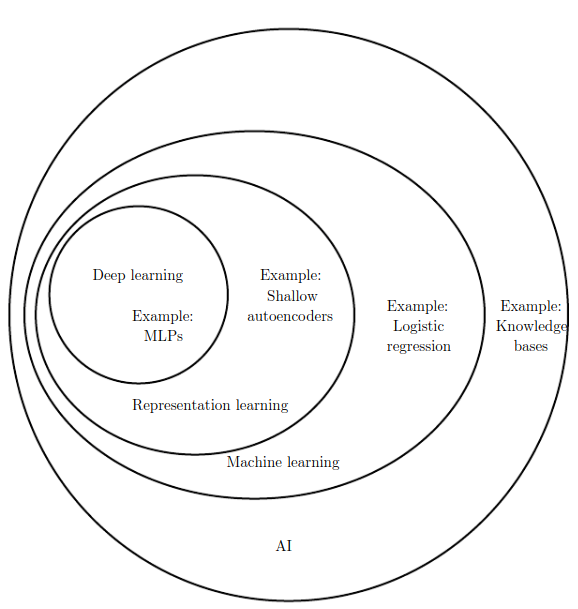
\includegraphics[width=0.7\textwidth,height=0.65\textheight,keepaspectratio]{images/marcoteorico/venn_diag}
		\vskip -2cm
		\end{center}
		\begin{center}
		\caption{\small{Diagrama de Venn donde cada sección incluye un ejemplo de una tecnología de IA(ilustra la relación entre estas diferentes disciplinas de la IA)}}
		\vskip -0.2cm
		{\small{Fuente: \citep{Goodfellow-et-al-2016}}}
		\end{center}

	\end{figure}
}

%	Para muchas tareas, sin embargo, es difícil saber qué características se deben extraer. Por ejemplo, un programa para detectar automóviles en fotografías. Se sabe que los autos tienen ruedas, por lo que sería importante utilizar la presencia de una rueda como característica. Desafortunadamente, es difícil describir exactamente cómo es una rueda en términos de valores de píxel. Una rueda tiene una geometría simple, pero su imagen puede verse complicada por las sombras que caen sobre la rueda, el sonido de las partes metálicas de la rueda, el guardabarros del automóvil o un objeto en el primer plano que oscurece la rueda, y así sucesivamente. 



\frame{
\begin{block}
{\Large{Aprendizaje Profundo}}
\end{block}
	
	\begin{itemize}
	\item<1->El aprendizaje profundo es un enfoque específico utilizado para construir y entrenar redes neuronales para la toma de decisiones altamente prometedoras, \citep{Goodfellow-et-al-2016}.

	\item<2->Se considera que un algoritmo es profundo si los datos de entrada se pasan a través de una serie de no linealidades o transformaciones no lineales antes de que se emita. 

	\item<3->Este enfoque permitir que las computadoras aprendan de la experiencia y entiendan el mundo en términos de una jerarquía de conceptos, con cada concepto definido a través de su relación con conceptos más simples. 

	\item<4->Al reunir el conocimiento de la experiencia, este enfoque evita la necesidad de que los operadores humanos especifiquen formalmente todo el conocimiento que necesita la computadora.
	\end{itemize}
}


\frame{
\begin{block}
{\Large{Aprendizaje Profundo}}
\end{block}
	\begin{figure}[H]
		\begin{center}
		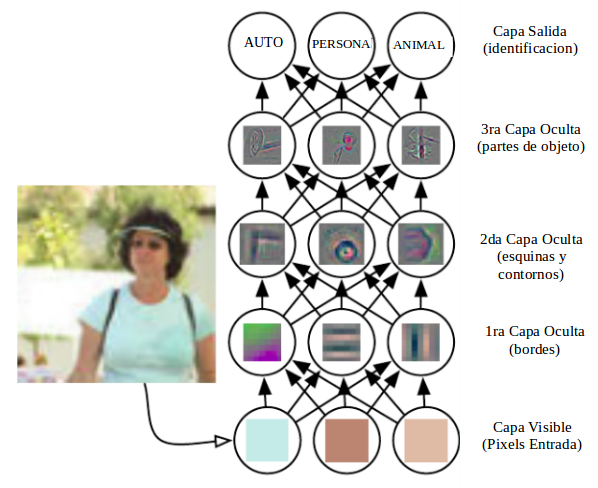
\includegraphics[width=0.7\textwidth,height=0.65\textheight,keepaspectratio]{images/marcoteorico/deepExam}
		\end{center}
		\vskip -0.5cm
		\begin{center}
		\caption{\small{El aprendizaje profundo permite a la computadora construir conceptos complejos a partir de conceptos más simples}}
		\vskip -0.2cm
		{\small{Fuente propia}}
		\end{center}
	\end{figure}
}


%-----------------%-----------------Red Convolucional-----------------%-----------------
\subsection{Red Convolucional}
\frame{
\begin{block}
{\Large{Red Convolucional}}
\end{block}

		\begin{itemize}
			\item<1->Nueve de cada diez veces, cuando se escucha que el aprendizaje profundo rompe una nueva barrera tecnológica, las redes neuronales convolucionales están involucradas. También llamados CNN(del inglés , {\bf Convolutional Neural Networks}) o  {\bf ConvNets}, estas son las preferidas del campo de redes neuronales profundas. Han aprendido a clasificar las imágenes en categorías incluso mejor que los humanos en algunos casos, \citep{Rohrer}.
			\vskip 0.5cm
			\item<2-> Estas son muy similares a las redes neuronales ordinarias, están formadas por neuronas que tienen pesos y biases(sesgos) que se pueden aprender durante el entrenamiento de estas. Cada neurona recibe algunas entradas y realiza operaciones matemáticas.
		\end{itemize}
}


\frame{
\begin{block}
{\Large{Red Convolucional}}
\end{block}
		\begin{itemize}
			\item<1->Una ConvNet se caracteriza por tener una secuencia de capas donde cada una de estas transforma un volumen de activaciones en otro nuevo a través de funciones y el aprendizaje profundo se produce cuando se utilizan varias de estas capas variando los parámetros de configuación dentro y entre dichas capas. 
			\vskip 0.5cm
			\item<2->El resultado de las CNNs es que pueden encontrar si una característica está en una imagen sin preocuparse exactamente de donde está. Esto ayuda a resolver el problema de las computadoras al comparar imágenes de manera hiper-literal, es decir, que coincida pixel a pixel para que se trate de imágenes iguales.
			%\vskip 0.5cm
		\end{itemize}
}




\frame{
\begin{block}
{\Large{Red Convolucional}}
\end{block}
		\begin{figure}[H]
		\begin{center}
		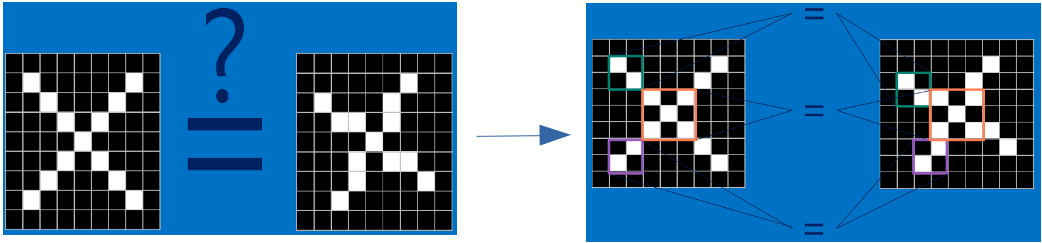
\includegraphics[width=0.8\textwidth]{images/marcoteorico/literalcomp}
		\end{center}
		\begin{center}
		\caption{\small{Analisis de una CNN}}
		\vskip -0.25cm
		{\small{Fuente: \citep{Rohrer}}}
		\end{center}
		\vspace{-1.5em}
		\end{figure}

}

%--------------------Red Convolucional - Terminologías-------------------------
\frame{
\begin{block}
{\Large{Red Convolucional}}
\end{block}
	\begin{itemize}
	\item<1-> {\bf Red Convolucional - Terminologías}
			\vskip 0.5cm
		\begin{itemize}
			\item<2->Una es cuando la red convolucional es vista como un número largo de capas simples y cada paso del procesamiento se considera como una capa en sí misma. 
			\vskip 0.5cm
			\item<3->Otra terminología es cuando la red convolucional es vista como un número pequeño de capas relativamente complejas, donde cada capa tiene multiples etapas.
			
		\end{itemize}
	\end{itemize}
}

\frame{
\begin{block}
{\Large{Red Convolucional}}
\end{block}
	\begin{itemize}
	\item<1-> {\bf Red Convolucional - Terminologías}
	
		\begin{figure}[H]
		\begin{center}
		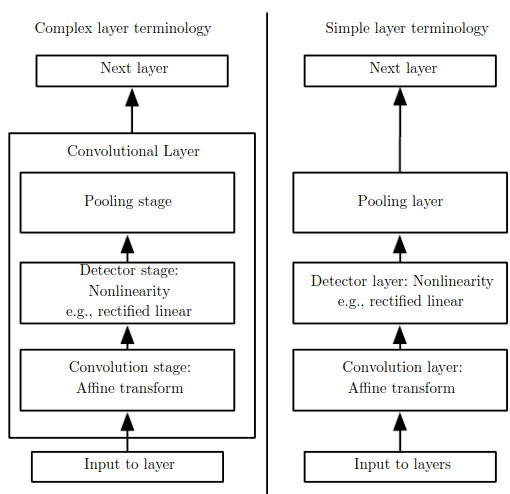
\includegraphics[width=0.6\textwidth,height=0.65\textheight,keepaspectratio]{images/marcoteorico/types}
		\end{center}
		
		\begin{center}
		\caption{\tiny{Terminología de capas complejas(izquierda) y de capas simples(derecha)}}
		\vskip -0.25cm
		{\tiny{Fuente: \citep{Goodfellow-et-al-2016}}}
		\end{center}
		%\vspace{-1.5em}
		\end{figure}
	\end{itemize}
}
%-----------------%----Arquitectura del Modelo-----%-----------------
\subsection{Arquitectura del Modelo}
\frame{
\begin{block}
{\Large{Arquitectura del Modelo}}
\end{block}
		\begin{itemize}
			\item<1->La arquitectura de la red está inspirada en el arquitectura Inception \citep{Inception} y en la arquitectura AlexNet\citep{Krizhevsky2012} para la clasificación de imágenes. En la arquitectura Inception, el modelo creado es denominado GoogLeNet, similar a AlexNet donde varios módulos iniciales son apilados uno sobre el otro para producir el resultado final. En el módulo de inicio, en ese tipo de red se usaron diversos tamaños de filtros convolucionales para capturar características de diferente abstracción. 
			\vskip 0.5cm
			\item<2-> El alto nivel de abstracción se captura con filtros de mayor tamaño y el de un nivel inferior con filtros de menor tamaño. Procesando información visual a diferentes escalas y al concatenarlas se obtiene un nivel eficiente de abstracción. 
		\end{itemize}
}



\frame{
\begin{block}
{\Large{Arquitectura del Modelo}}
\end{block}
		\begin{itemize}
		\vskip 0.5cm
		\item<1-> En esta investigación se utilizó una versión modificada de las arquitecturas antes mencionadas. Se incorporó {\bf funciones de escala-múltiple} \citep{Multi_scale_feat}, lo que significa que la salida de las capas convolucionales no solo se envía a la capa posterior, sino que también se ramifica y se introduce al clasificador (capa totalmente conectada). La razón detrás de esto es que cuando el clasificador está tomando una decisión basada en convoluciones, podría encontrar que la salida de la primera o segunda capa convolucional también es útil. Básicamente con las características de escala múltiple depende del clasificador qué nivel de abstracción usar, ya que tiene acceso a las salidas de todas las capas convolucionales, es decir, características en todos los niveles de abstracción.

		% Estas capas ramificadas se someten a un pooling máximo adicional, de modo que todas las convoluciones se submuestrean proporcionalmente antes de entrar en el clasificador. Así se garantiza que todas las funciones de escala múltiple experimenten la misma cantidad de máximo aprovechamiento.

		\end{itemize}
}


\frame{
\begin{block}
{\Large{Arquitectura del Modelo}}
\end{block}
		\begin{figure}[H]
		%\begin{center}
		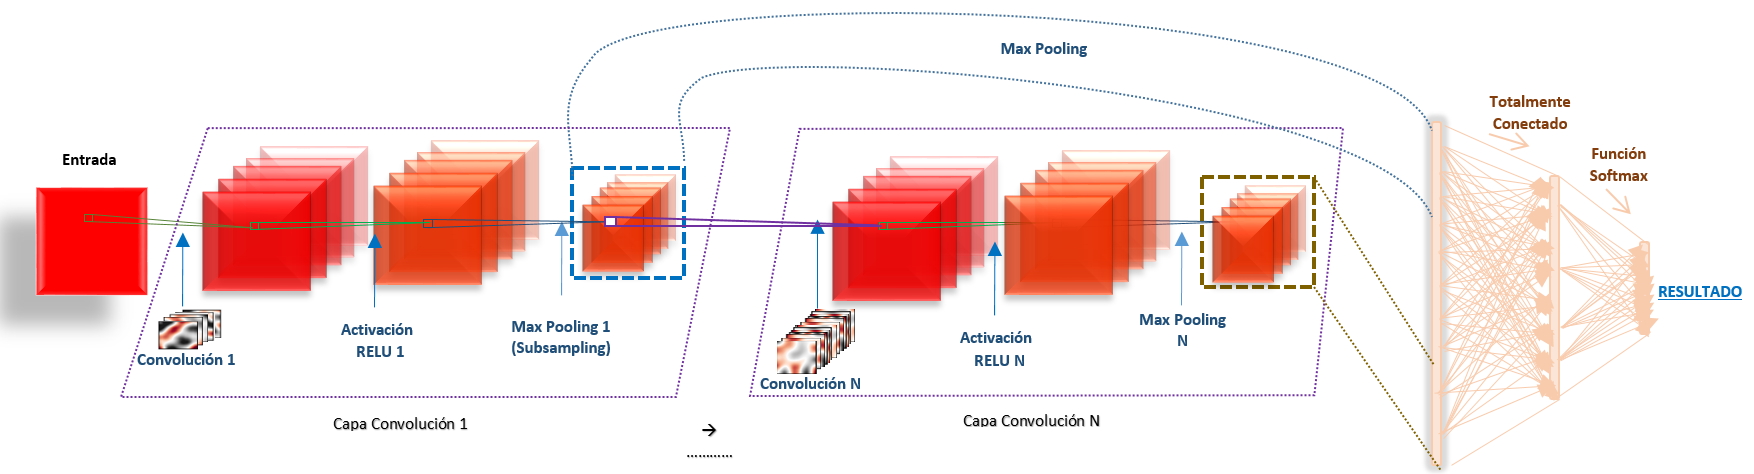
\includegraphics[width=1\textwidth]{images/desarrollo/networkArquitec/designNet}
		%\end{center}
		\begin{center}
		\caption{\small{Modelo del diseño de la Red propuesta}}
		
		{\small{\fontsize{10}{16.8}\selectfont {Fuente propia}}}
		\end{center}
		\vspace{-1.5em}
		\end{figure}
}


%-----------------%----Componentes del Modelo-----%-----------------
\subsection{Componentes del Modelo}
\frame{
\begin{block}
{\Large{Componentes del Modelo}}
\end{block}
		\begin{itemize}
			\item<1->Capa Convolucional
			\vskip 0.5cm
			\item<2-> Capa de Activación ReLU(Rectified Linear Units)
			\vskip 0.5cm
			\item<3-> Capa de Agrupación(Pooling)
			\vskip 0.5cm
			\item<4-> Capa totalmente conectada (Fully-connected layer)
		\end{itemize}
}
%--------------------------------------Capa Convolucional------------------------------
%\subsubsection{Capa Convolucional}
\frame{
\begin{block}
{\Large{Capa Convolucional}}
\end{block}
		\begin{itemize}
			\item<1->Los parámetros de la capa convolucional consisten basicamente en dos datos. La entrada y todo lo que respecta a un conjunto de filtros(también denomidados kernels) cuyos valores se aprenden, es decir, empiezan con datos aleatorios y conforme avance el entrenamiento se van alterando. 
			\vskip 0.5cm
			\item<2-> Durante el proceso hacia adelante, se desliza (más precisamente, convolve) cada filtro a través del ancho y alto del volumen de entrada para calcular los productos de puntos entre las entradas del filtro y la entrada en cualquier posición.
		\end{itemize}
}

\frame{
\begin{block}
{\Large{Capa Convolucional}}
\end{block}

		\begin{figure}[H]
			\begin{center}
			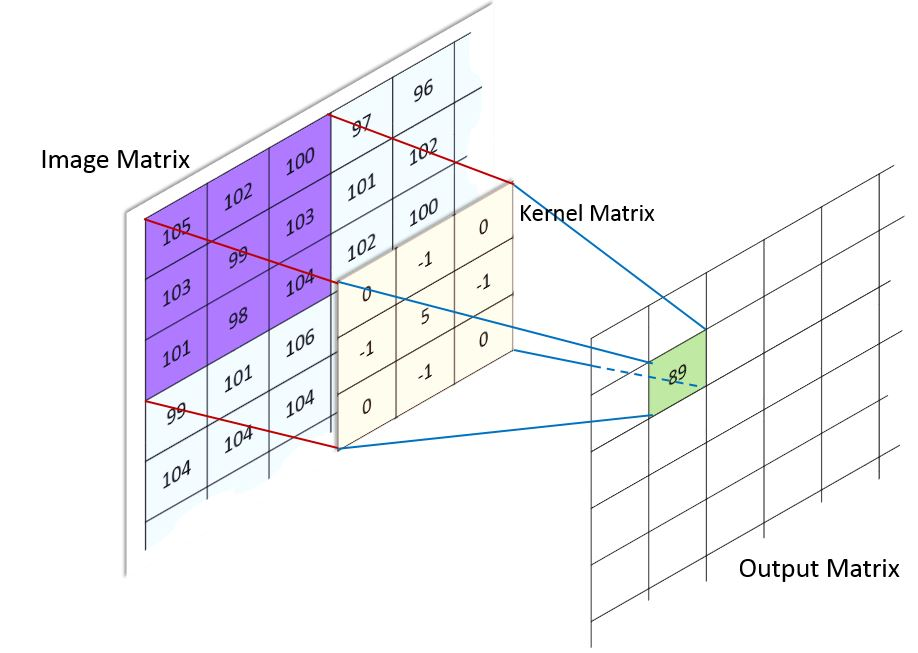
\includegraphics[width=0.75\textwidth,height=0.5\textheight,keepaspectratio]{images/marcoteorico/Convolution_calculation1}
			\end{center}
			\begin{center}
			\caption{\tiny{Posicionamiento del kernel/filtro por pixel}}
			{\tiny{Fuente: Fuente Propia}}
			\end{center}
			
		\end{figure}
}


\frame{
\begin{block}
{\Large{Capa Convolucional}}
\end{block}

		\begin{itemize}
			\item<1->A medida que deslizamos el filtro sobre el ancho y la altura del volumen de entrada produciremos un mapa de activación bidimensional que proporciona las respuestas de ese filtro en cada posición espacial. Por lo que simplemente se multiplica cada píxel en el filtro por el valor del píxel en la imagen. Para luego, sumar las respuestas y dividirlas por el número total de píxeles en el filtro. 
		
		%\item<3->
		\begin{figure}[H]
		\begin{center}
		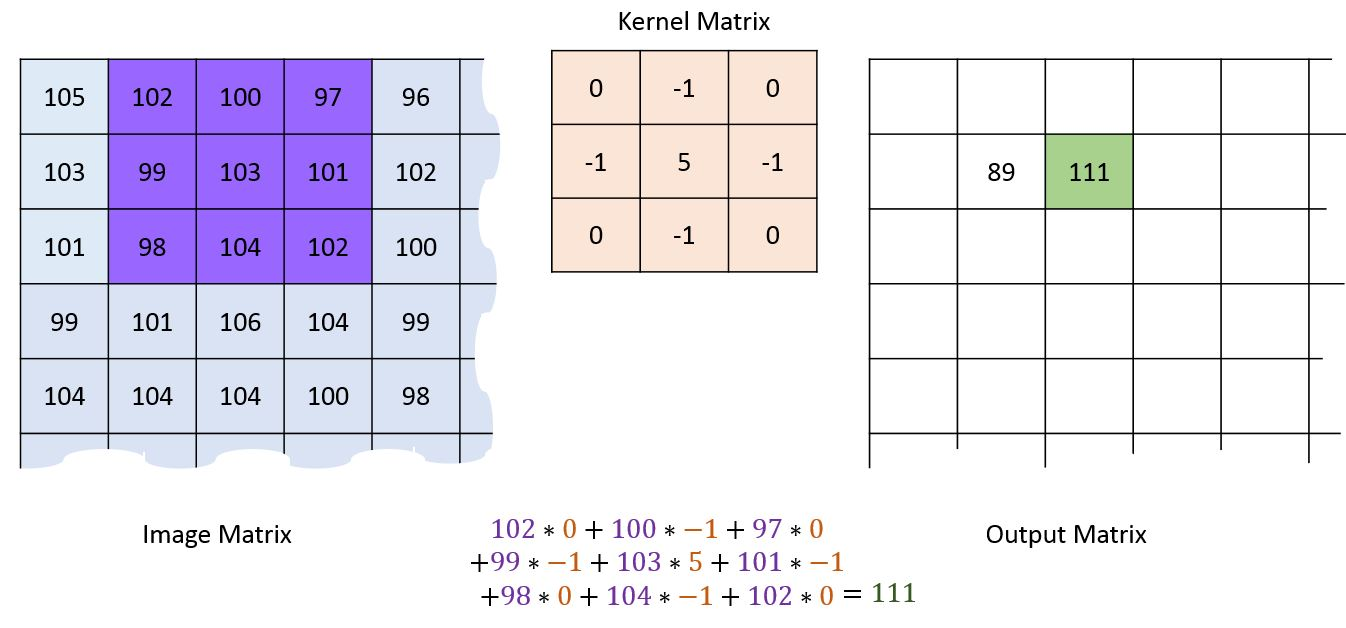
\includegraphics[width=0.75\textwidth,height=0.4\textheight,keepaspectratio]{images/marcoteorico/Convolution_calculation2}
		\end{center}
		\begin{center}
		\caption{\tiny{Cálculo Convolucional}}
		{\tiny{Fuente: Fuente Propia}}
		\end{center}
		
		\end{figure}

		\end{itemize}
}


\frame{
\begin{block}
{\Large{Capa Convolucional}}
\end{block}

		\begin{itemize}
			\item<2->Intuitivamente, la red aprenderá los filtros que se activan cuando ven algún tipo de característica visual, como un borde o contorno en alguna orientación específica. Debido a que la convolución aprovecha tres ideas importantes que pueden ayudar a mejorar un sistema de aprendizaje automático: 
			\begin{itemize}
			\item<3-> Interacciones dispersas
			\item<4-> Uso compartido de parámetros
			\item<5-> Representaciones equivalentes
			\end{itemize}
		\end{itemize}

}

\frame{
\begin{block}
{\Large{Capa Convolucional}}
\end{block}
		\begin{itemize}
	\item<1-> {\bf Capa Convolucional - Interacciones dispersas}
	%\vskip 0.5cm
			\begin{figure}[H]
		\begin{center}
		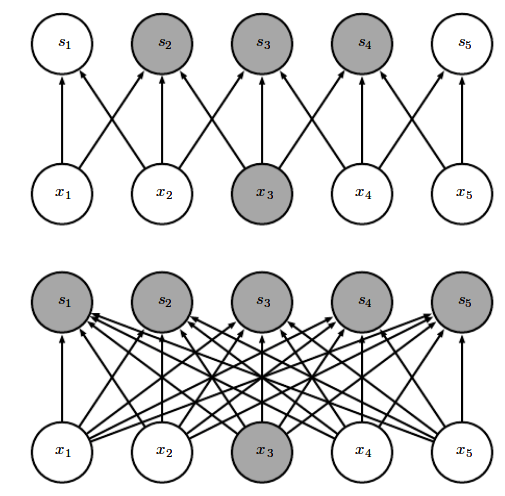
\includegraphics[width=0.5\textwidth,height=0.4\textheight,keepaspectratio]{images/marcoteorico/sparceCon}
		\end{center}
		
		\begin{center}
		\caption{\footnotesize \small{Conectividad dispersa vs No dispersa}}
		\vskip -0.3cm  
		{\small{Fuente:\citep{Rohrer}}}
		\end{center}
		\end{figure} 
		 Cuando {\bf {\textit {s}}} está formado por convolución con un kernel de ancho 3, solo tres salidas se ven afectadas por {\bf \textit  x}. (Abajo) Cuando {\bf \textit s} está formado por la multiplicación de la matriz, la conectividad ya no es dispersa, por lo que todos los resultados se ven afectados por $x_{3}$.
	\end{itemize}
}

\frame{
\begin{block}
{\Large{Capa Convolucional}}
\end{block}
		\begin{itemize}
	\item<1-> {\bf Capa Convolucional - Interacciones dispersas}
	 	\begin{itemize}
	 		\vskip 0.5cm
	 	\item<2->Esto significa que necesitamos almacenar menos parámetros, lo que reduce los requisitos de memoria del modelo y mejora su eficiencia estadística. También significa que el cálculo de la salida requiere menos operaciones, \citep{Goodfellow-et-al-2016}.
		\end{itemize}
	\end{itemize}
}

\frame{
\begin{block}
{\Large{Capa Convolucional}}
\end{block}
		\begin{itemize}
	\item<1-> {\bf Capa Convolucional - Uso compartido de parámetros}
	 	\begin{itemize}
	 		\vskip 0.5cm
	 	\item<2->En una red neuronal convolucional, cada miembro del kernel se utiliza en cada posición de la entrada (excepto tal vez algunos de los píxeles de los bordes, dependiendo de las decisiones de diseño con respecto al límite). El uso compartido de parámetros utilizado por la operación de convolución significa que en lugar de aprender conjuntos de parámetros para cada ubicación por separado, aprendemos un solo conjunto por kernel, \citep{Goodfellow-et-al-2016}.
		\end{itemize}
	\end{itemize}
}

\frame{
\begin{block}
{\Large{Capa Convolucional}}
\end{block}
		\begin{itemize}
	\item<1-> {\bf Capa Convolucional - Representaciones equivalentes}
	 	\begin{itemize}
	 		\vskip 0.5cm
	 	\item<2->La forma particular de compartir los parámetros hace que la capa tenga una propiedad llamada {\bf representaciones equivalentes}. Decir que una función es equivalente significa que si la entrada cambia, la salida cambia de la misma manera.
	 	\vskip 0.3cm
	 	\item<3->La convolución crea un mapa en 2-D de donde aparecen ciertas características en la entrada. Si movemos el objeto en la entrada, su representación se moverá la misma cantidad en la salida.
		\end{itemize}
	\end{itemize}
}

%Por ejemplo, al procesar imágenes, es útil detectar bordes en la primera capa de una red convolucional. Los mismos bordes aparecen más o menos en todas partes en la imagen, por lo que es práctico compartir los parámetros en toda la imagen.


\frame{
\begin{block}
{\Large{Capa Convolucional}}
\end{block}
	\begin{itemize}
	\item<1-> {\bf Capa Convolucional - Representaciones equivalentes}
	 	\begin{figure}[H]
		\begin{center}
		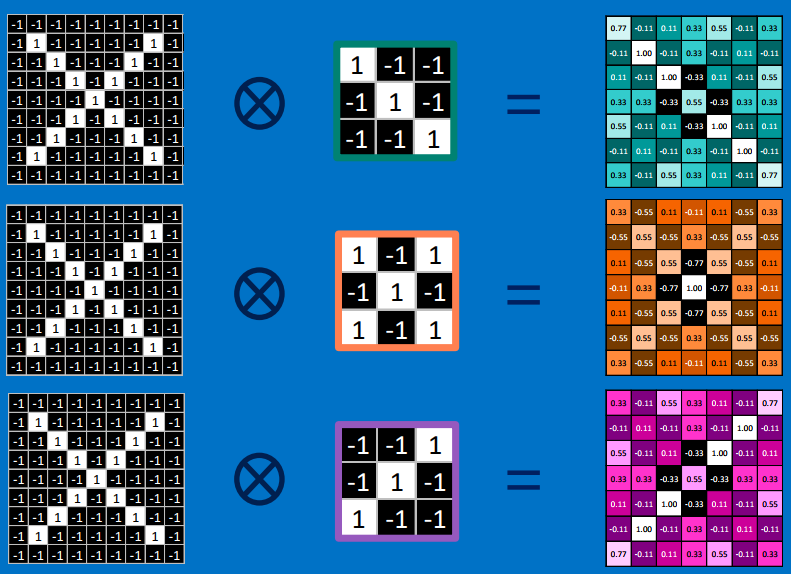
\includegraphics[width=0.6\textwidth,height=0.4\textheight,keepaspectratio]{images/marcoteorico/result_conv}
		\end{center}
		\begin{center}
		\vskip 0.1cm  
		\caption{\small{Resultado de Convolución(conjunto de mapas de activación. generado a partir de 3 filtros para 3 carecteristicas: diagonal derecha, cruzamiento central y diagonal izquierda). Simbolo de convolución: $\otimes$}}
		\vskip -0.1cm  
		{\small{Fuente: \citep{Rohrer}}}
		\end{center}
		\end{figure}

	\end{itemize}
}

%-----------------------------------------------------------------------------------

\frame{
\begin{block}
{\Large{Capa Convolucional}}
\end{block}
	\begin{itemize}
	\item<1-> {\bf Capa Convolucional - Construcción de un filtro o kernel}
		\setbeamertemplate{enumerate items}[square]
		\setbeamercolor{item projected}{bg=green!70!black,fg=blue}
	 	\begin{enumerate}
			\item La extensión espacial es el tamaño del filtro, comúnmente es de tamaño impar tanto en largo y ancho.
			
			\item El stride es otra pieza del bloque de construcción básico de los filtros convolucionales. Este representa el {\textit 'paso'} en la operación de convolución indicando cuánto es que se debe desplazar un filtro en una imagen con cada paso. El filtro se desliza sobre la imagen, se detiene en cada longitud de salto y realiza las operaciones necesarias en ese paso.

				\begin{figure}[H]
				\begin{center}
				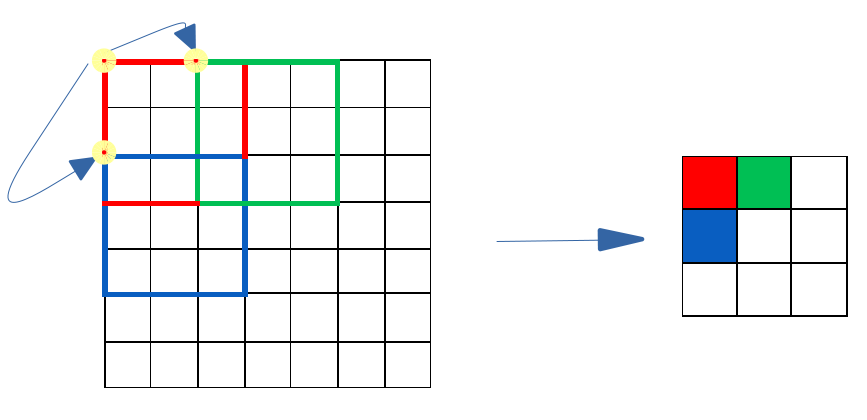
\includegraphics[width=0.65\textwidth,height=0.3\textheight,keepaspectratio]{images/marcoteorico/stride}
				\end{center}
				\begin{center}
				\caption{\tiny{Imagen con stride igual a 2, para el filtro tanto en largura como anchura}}
				\vspace{-0.5em}
				{\tiny{Fuente propia}}
				\end{center}
				\end{figure}
			\end{enumerate}
	\end{itemize}
}

\frame{
\begin{block}
{\Large{Capa Convolucional}}
\end{block}
	\begin{itemize}
	\item<1-> {\bf Capa Convolucional - Construcción de un filtro o kernel}
	 	\setbeamertemplate{enumerate items}[square]
	 	\setbeamercolor{item projected}{bg=green!70!black,fg=blue}
	 	\begin{enumerate}\addtocounter{enumi}{2}
			\item Zero-padding agrega ceros alrededor del borde de una imagen.
				\begin{figure}[H]
				\begin{center}
				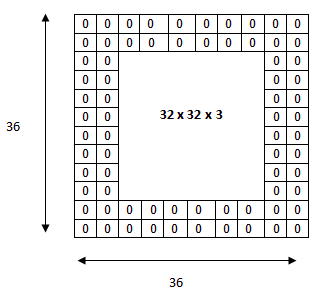
\includegraphics[width=0.4\textwidth]{images/marcoteorico/PAD2}
				\end{center}
				\begin{center}
				\caption{\tiny{Ejemplo de zero-padding con tamaño 2}}
				\vspace{-0.5em}
				{\tiny{Fuente propia}}
				\end{center}
				\end{figure}
		\end{enumerate}
	\end{itemize}
}

%Los principales beneficios del relleno son los siguientes:
%\item Le permite usar una capa de convolución sin necesariamente reducir la altura y el ancho de los volúmenes. Esto es importante para construir redes más profundas, ya que de lo contrario la altura / ancho se reduciría a medida que se avanza hacia capas más profundas.
%\item Nos ayuda a mantener más información en el borde de una imagen. Sin relleno, muy pocos valores en la siguiente capa se verían afectados por los píxeles como los bordes de una imagen.

\frame{
\begin{block}
{\Large{Capa Convolucional}}
\end{block}
		\begin{itemize}
		\item<1-> {\bf Capa Convolucional - Ecuación de Convolución}
	

	 	\vskip 0.5cm
	 	\item<2->	
		\begin{center}
		${conv_j^n} ={\sum_{k=1}^k x_k^n \times w_{kj} ^n + b_n}$
		\end{center}
		
		En el que:\vskip 0.1cm
		\begin{itemize}
			\item $x$ son valores de entrada
			\item $w,b$ pesos y biases(sesgos) del kernel, respectivamente
			\item $n$ es el número de la capa
			\item $j$ es el número del filtro de salida
			\item $k$ es la cantidad de filtros en la capa $n-1$ o $n$
		\end{itemize}

		
	\end{itemize}
}

\end{document}